\section{Que permet de faire l'intelligence artificielle~?}

Afin de pouvoir répondre à la problématique <<~\sujet ~>>, il faut prendre connaissance d'où en est l'état de l'art de l'intelligence artificielle.
Nous allons voir par la diversité des concepts avancés dans cette partie que l'intelligence artificielle est un domaine extrêmement vaste et qui permet des applications dans tous les domaines de l'industrie et de la recherche.

\subsection{Systèmes multi-agents}

Dans les systèmes multi-agents, des agents aux comportements individuels simples interagissent entre eux pour résoudre des problèmes complexes, par l'apparition d'une forme d'intelligence collective.

\subsubsection{Automates cellulaires}

Les automates cellulaires sont des outils permettant de mimer des processus auto-reproductifs (c'est un cas particulier de système multi-agents).
Ils sont basés sur des règles simplistes et permettent cependant de faire émerger des comportements extrêmement complexes.
Un automate cellulaire consiste en une grille de <<~cellules~>>, chaque cellule possède un état au temps $t$ et l'état de cette cellule au temps \textit{t+1} est défini par l'état des cellules avoisinantes au temps $t$ en fonction des règles définies.

L'exemple d'automate cellulaire le plus célèbre est le <<~jeu de la vie~>> imaginé par John Horton \textsc{Conway} en 1970 \cite{conway}.
Ce <<~jeu~>> se déroule sur une grille bi-dimensionnelle, les cases de celles-ci sont nommées des cellules et peuvent prendre deux états~:~<<~vivante (1)~>> ou <<~morte (0)~>>.
Les règles sont définies telles que~:~
\\
\begin{itemize}
    \item[\tiny$\bullet$] Une cellule morte possédant exactement trois voisines vivantes devient vivante, sa valeur passe à 1.
    
    \item[\tiny$\bullet$] Une cellule vivante possédant deux ou trois voisines vivantes le reste, sinon elle meurt.
\end{itemize}
~\\

La grille est ensuite initialisée, soit avec des valeurs pré-définies, soit aléatoirement.
L'univers généré paraît chaotique pendant quelques étapes, puis rapidement des structures apparaissent. Certaines sont stables, l'état des cellules les constituant ne change pas tant qu'aucun événement extérieur ne vient les perturber.
D'autres sont périodiques, l'état des cellules les constituants évolue au cours du temps et finit toujours par revenir au même point.
D'autres prennent la forme de vaisseaux, celles-ci sont capables de reproduire une copie d'elle-même après un certain nombre d'étapes, mais décalée dans l'univers du jeu.

La figure ci-dessous représente un \textsc{Gosper} glider gun, sa partie principale se répète périodiquement et émet des vaisseaux à intervalles réguliers.

\FloatBarrier
\begin{figure}[h!]
    \begin{minipage}[c]{0.55\textwidth}
        \begin{center}
            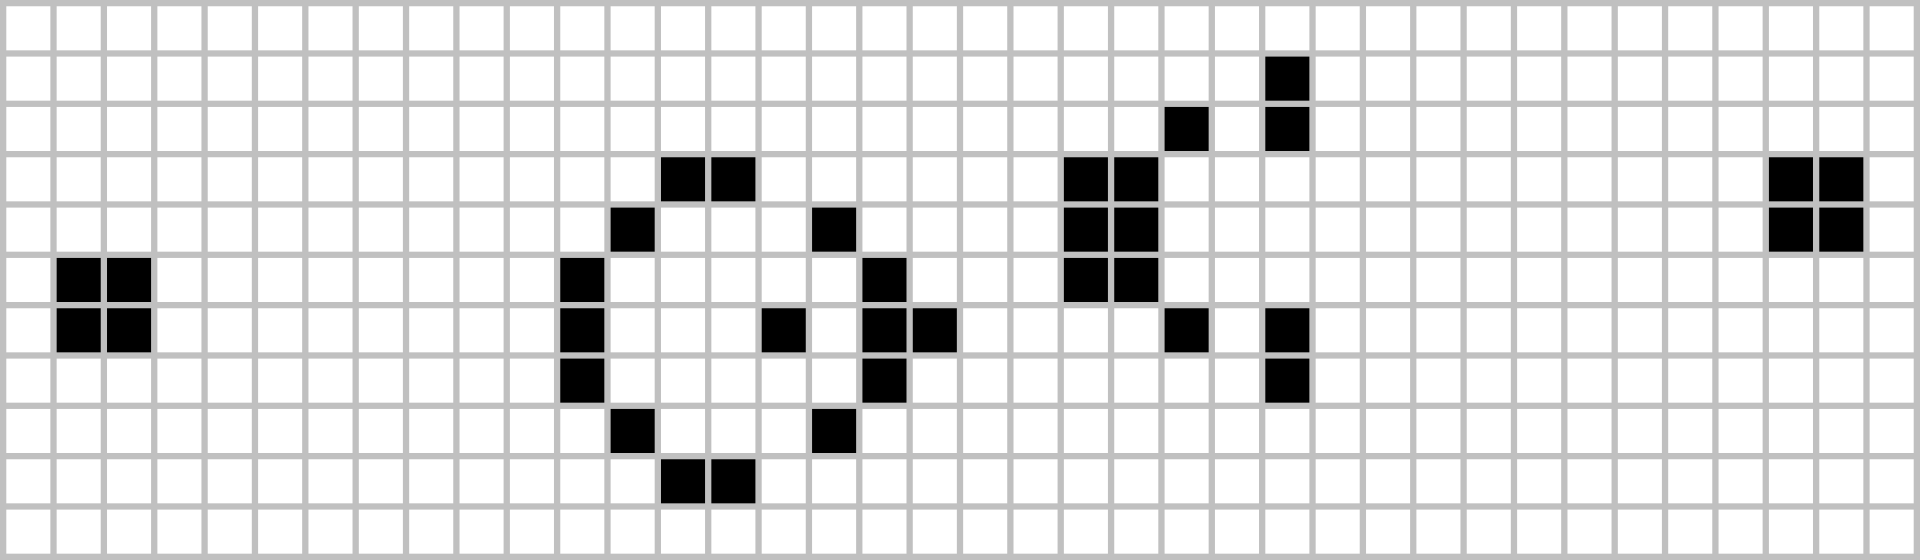
\includegraphics[width = 0.9\textwidth]{game_of_life_glider_gun}
        \end{center}
    \end{minipage}\hfill
    \begin{minipage}[c]{0.45\textwidth}
        \caption{\textsc{Gosper} glider gun}
        \label{figure:gun}
    \end{minipage}
\end{figure}
\FloatBarrier

Les automates cellulaires sont un exemple de systèmes constitués de composantes connues, mais faisant émerger des comportements bien plus complexes à appréhender.
Ils sont donc particulièrement utiles pour mener des recherches concernant des systèmes de propagation encore peu compris.
Dans une recherche de 2015, des chercheurs ont utilisé des automates cellulaires afin de modéliser et simuler la propagation et l'évolution de maladies \cite{cellular_automata_diseases}.
Dans une autre étude de 2019 ils sont utilisés pour simuler la propagation d'incendies de forêt \cite{cellular_automata_fire}.

\subsubsection{Simulation de foules}

On utilise les systèmes multi-agents pour simuler des interactions existant entre agents autonomes.
Le but est de déterminer l'évolution de ce système afin de prévoir l'organisation qui en résulte.
Ils permettent notamment d'expérimenter des scénarios qui ne seraient pas réalisables sur des populations réelles, que ce soit pour des raisons techniques ou éthiques.
Ce qui importe c'est le comportement d'ensemble et non pas le comportement individuel.

Ils sont par exemple utilisés dans le monde de l'industrie, dans les jeux vidéo et dans l'animation, avec notamment le logiciel \textsc{Massive} (Multiple Agent Simulation System in Virtual Environment, littéralement <<~Système de simulation multi-agents dans un environnement virtuel~>>).
Celui-ci permet de simuler des foules.
Il a été développé à l'occasion de la trilogie cinématographique du Seigneur des Anneaux et est utilisé dans de nombreux films.

Ils sont aussi utilisés dans le monde de la recherche, par exemple, pour l'analyse de mouvements de foules, de mouvements de paniques, du trafic routier, de la propagation de maladies, etc.

Ci-dessous est un exemple de système multi-agents développé de manière à simuler des poissons formant des bancs.
Sur cette image les traits fins sont des agents qui sont effrayés par les agents représentés par des traits épais.
On peut voir apparaître des comportements de formation de bancs organisés par type d'agent (gros sur la droite et petits sur la gauche) et un comportement de fuite qui s'amorce de la part des petits poissons devant l'arrivée du banc de gros poissons.
Cette image est extraite d'un de mes projets personnels \cite{fish_shoal}.

\FloatBarrier
\begin{figure}[h!]
    \begin{minipage}[c]{0.55\textwidth}
        \begin{center}
            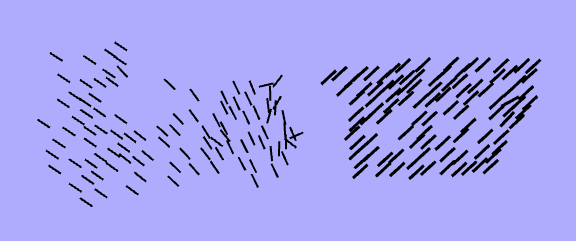
\includegraphics[width = 0.9\textwidth]{little_big}
        \end{center}
    \end{minipage}\hfill
    \begin{minipage}[c]{0.45\textwidth}
        \caption{Formation de deux bancs de poissons organisés par <<~espèces~>>}
        \label{figure:shoal}
    \end{minipage}
\end{figure}
\FloatBarrier

Il est intéressant de constater que lorsqu'une minorité des petits poissons est capable de voir le danger arriver et commence à fuir, c'est la totalité du banc qui débute un demi-tour.
C'est ce genre de comportement qui permet à des poissons réels, tels que les sardines, d'augmenter les chances de survies d'un maximum d'individus en cas d'attaque d'un prédateur.

\subsection{Algorithmes génétiques}\label{section:ga}

Les algorithmes génétiques sont inspirés du processus de sélection naturelle et permettent d'obtenir une ou plusieurs solutions répondant à un problème d'optimisation.

Initialement, une population est générée aléatoirement, où chaque individu représente une solution du problème.
Les individus possèdent un génome qui leur est propre, c'est celui-ci qui définit les caractéristiques de chacun.
Une sélection est ensuite effectuée parmi la population afin de ne sélectionner que les plus performants.
Lorsque deux individus sont sélectionnés, un entrecroisement (ou cross-over) est effectué sur leurs génomes.
Ce croisement est une simulation d'un phénomène génétique qui contribue au brassage génétique lors de la reproduction.
Ce croisement entraîne la création d'un nouveau génome, sur lequel on peut appliquer des mutations aléatoires.
Ainsi, une nouvelle population est générée à partir de la précédente, c'est donc une nouvelle génération.
Ce processus est ensuite répété de nombreuses fois afin de simuler le principe d'évolution.
À terme, les individus deviennent plus performants et tendent vers la solution optimale pour la résolution du problème posé.

Les problèmes pouvant être traités à l'aide de ce type d'algorithmes sont très variés, leur domaine d'application le plus impressionnant est sans doute l'optimisation de designs.
La solution logicielle <<~Generative Design~>>, de la compagnie \textsc{Autodesk}, permet à un utilisateur de définir ses besoins en termes d'aérodynamisme, de solidité, de type de matière, etc.
Le logiciel utilise ensuite un système d'algorithme génétique pour générer un ensemble de possibilités répondant aux besoins, qu'il propose à l'utilisateur.
Le logiciel permet de générer des formes complexes permettant de mieux répondre aux contraintes que n'importe quel design qu'un être humain aurait pu imaginer.

\FloatBarrier
\begin{figure}[h!]
    \begin{minipage}[c]{0.4\textwidth}
        \begin{center}
            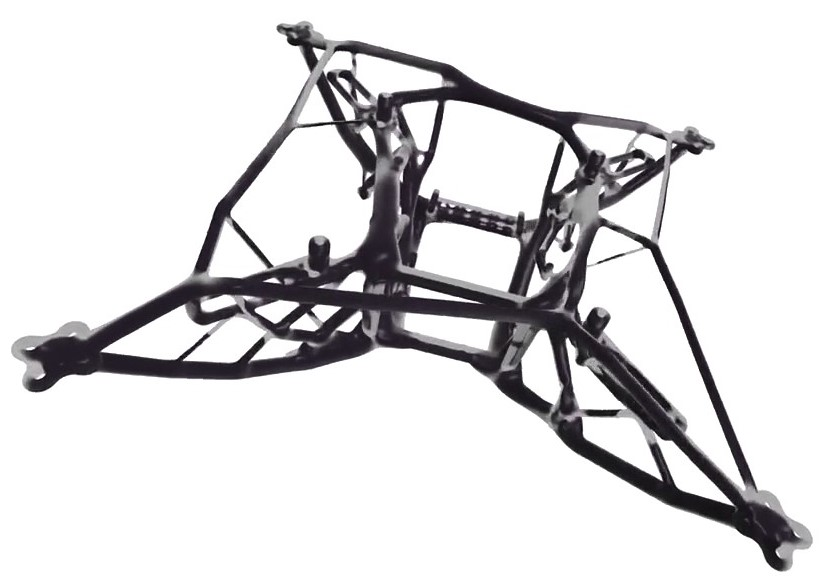
\includegraphics[width = 0.9\textwidth]{ga_drone}
        \end{center}
    \end{minipage}\hfill
    \begin{minipage}[c]{0.5\textwidth}
        \caption{Châssis de drone léger et résistant, généré et proposé par Generative Design}
        \label{figure:drone}
    \end{minipage}
\end{figure}
\FloatBarrier

\subsection{Recherche de chemin}

Le problème de la recherche de chemin consiste à trouver une solution pour se déplacer dans un environnement entre un point de départ et un point d'arrivée en prenant en compte différentes contraintes.

Il existe des algorithmes de recherche de chemin très célèbres, avec notamment l'algorithme de Dijkstra et l'algorithme A*.
Le premier est utilisé pour déterminer un chemin optimal, il est par exemple utilisé dans la pratique dans des protocoles de routage au sein de réseaux informatiques.
Le second présente l'avantage d'être plus rapide, mais n'offre cependant pas la certitude de l'optimalité.

Les algorithmes de recherche de chemin sont énormément utilisés dans le domaine de la robotique mobile et dans le domaine du jeu vidéo dans lesquels des entités doivent se déplacer.

À un niveau plus avancé, les outils de GPS, tels que Google Maps, utilisent aussi des algorithmes de recherche de chemin qui sont appliqués à une transformation de la carte sous forme de graphe.

\subsection{Modèles de \textsc{Markov} cachés}

Un modèle de \textsc{Markov} caché est un modèle statistique dans lequel le système modélisé est supposé être un processus de \textsc{Markov} de paramètres inconnus.
C'est un processus stochastique possédant la propriété de \textsc{Markov}.
Cette propriété est vérifiée si et seulement si la distribution conditionnelle de probabilité des états futurs ne dépend que de l'état présent et non pas des états passés.
Concrètement, c'est un système sans mémoire.

Les modèles de \textsc{Markov} cachés sont beaucoup utilisés en classification d'images \cite{hmm_classification}, segmentation d'images \cite{hmm_segmentation}, traitement automatique du langage naturel \cite{hmm_speech}, ou encore en modélisation de séquences en biologie \cite{hmm_bio}.

\subsection{L'apprentissage profond}

L'apprentissage profond, appelé deep learning en anglais, est un ensemble de méthodes d'apprentissage automatique (machine learning) dont le but est de modéliser des données à un fort niveau d'abstraction afin de répondre à des problèmes complexes.
Ces méthodes ne furent mises en pratique que récemment, grâce à la forte amélioration des capacités de calcul des ordinateurs.
Elles ont permis des avancées spectaculaires dans les domaines de l'analyse de signaux sonores ou visuels et notamment de la reconnaissance faciale, vocale, de la vision par ordinateur, du traitement automatique du langage, etc.
Les méthodes d'apprentissage profond suscitèrent l'intérêt de l'industrie dans les années 2000, avec notamment les GAFA (\textsc{Google}, \textsc{Apple}, \textsc{Facebook} et \textsc{Amazon}), ce qui a permis des avancées très rapides ces dernières années.

Cette section n'est absolument pas une liste exhaustive de tous les concepts existants dans le domaine de l'apprentissage profond, cependant, les concepts les plus utilisés et donnant lieu aux plus grandes avancées sont abordés via la présentation d'une ou plusieurs de leurs applications.

\subsubsection{L'émergence d'agents coopératifs complexes}

Le 30 mai 2019, la société \textsc{DeepMind}, détenue par la société \textsc{Alphabet}, a présenté un système multi-agent capable de jouer au jeu <<~Quake III Arena Capture the Flag~>> avec des performances supérieures à celles d'excellents joueurs \cite{deepmind_ctf}.

Dans ce jeu il y a deux équipes, chaque équipe possède une base dans laquelle se trouve un drapeau à leur couleur respective.
Le but de chaque équipe est de coopérer pour aller voler le drapeau adverse afin de le ramener à la base alliée, tout en défendant le drapeau allié.
Les joueurs peuvent aussi tirer sur ceux de l'équipe adverse afin de les faire réapparaître dans leur base.
Les règles sont simples, mais la dynamique de jeu entre les équipes est complexe.

Dans le monde réel, chaque humain possède ses propres objectifs et possibles actions, mais nous sommes tout de même capables de nous allier pour former des équipes, des sociétés, en présentant une intelligence collective impressionnante.
C'est quelque chose qui est appelé l'apprentissage multi-agent, c'est un problème extrêmement complexe, car avec des agents apprenants tous en parallèle, le monde évolue constamment.
Afin d'investir ce problème, beaucoup de scientifiques s'intéressent aux jeux vidéo 3D multijoueurs à la première personne.
Le fait que ces jeux soient à la première personne complexifie beaucoup le problème, car la vision du monde n'est pas omnisciente.
L'environnement est vu du point de vue d'un individu unique.
Il faut donc être capable de créer une représentation imaginaire de l'environnement non observable afin de pouvoir anticiper un maximum de situations.

Dans cette expérience, les agents de \textsc{DeepMind} ont dû apprendre, à partir de rien, comment voir, agir et coopérer dans un environnement vu à la première personne, le tout avec pour seule indication de leur performance le score de l'équipe.
L'apprentissage est basé sur le principe d'apprentissage par renforcement, c’est-à-dire que l'on indique à l'agent si sa performance est bonne ou mauvaise et celui-ci en tire une expérience lui permettant de s'améliorer.

Le fonctionnement de chaque agent est basé sur un réseau de neurones récurrents.
Contrairement à un réseau de neurones classique (qui nécessite des données d'entrées ayant une taille définie bien précise), ces derniers sont adaptés pour des données d'entrées de taille variable, en particulier pour des séries temporelles.
Ils sont utilisés dans la reconnaissance de la parole ou de l'écriture manuscrite par exemple.
Ce genre de réseau est adapté dans ce cas, car les agents doivent effectuer des actions en réponse à des séries d'actions effectuées par leurs alliés et les ennemis, il leur faut donc un semblant de mémoire des actions effectuées auparavant.

Pour entraîner les agents, ceux-ci jouent en équipes d'agents contre agents et apprennent tout d'eux-mêmes, ils sont capables d'apprendre seuls des tactiques connues des joueurs de haut niveau.
Les agents ainsi entraînés sont aussi capables de s'adapter pour jouer sur des cartes inconnues et même à d'autres modes de jeux.

\subsubsection{AlphaStar}

Le 19 janvier 2019, AlphaStar bat le joueur Grzegorz \textsc{Komincz}, appelé <<~MaNa~>> et l'un des meilleurs joueurs du monde, 5 parties à 0, sur le jeu StarCraft II \cite{alphastar}.
AlphaStar est développé par la société \textsc{DeepMind}.
StarCraft II est aujourd'hui considéré comme étant le jeu de stratégie en temps réel le plus complexe au monde et est devenu récemment l'un des <<~grands challenges~>> de l'intelligence artificielle.
Le mode de jeu le plus célèbre, et celui sur lequel AlphaStar est entraîné est le mode 1v1, c'est-à-dire deux joueurs qui s'affrontent l'un contre l'autre, chacun devant construire sa base dans l'objectif de produire le plus de ressources possible tout en optimisant sa défense et son attaque.

\FloatBarrier
\begin{figure}[h!]
    \begin{center}
        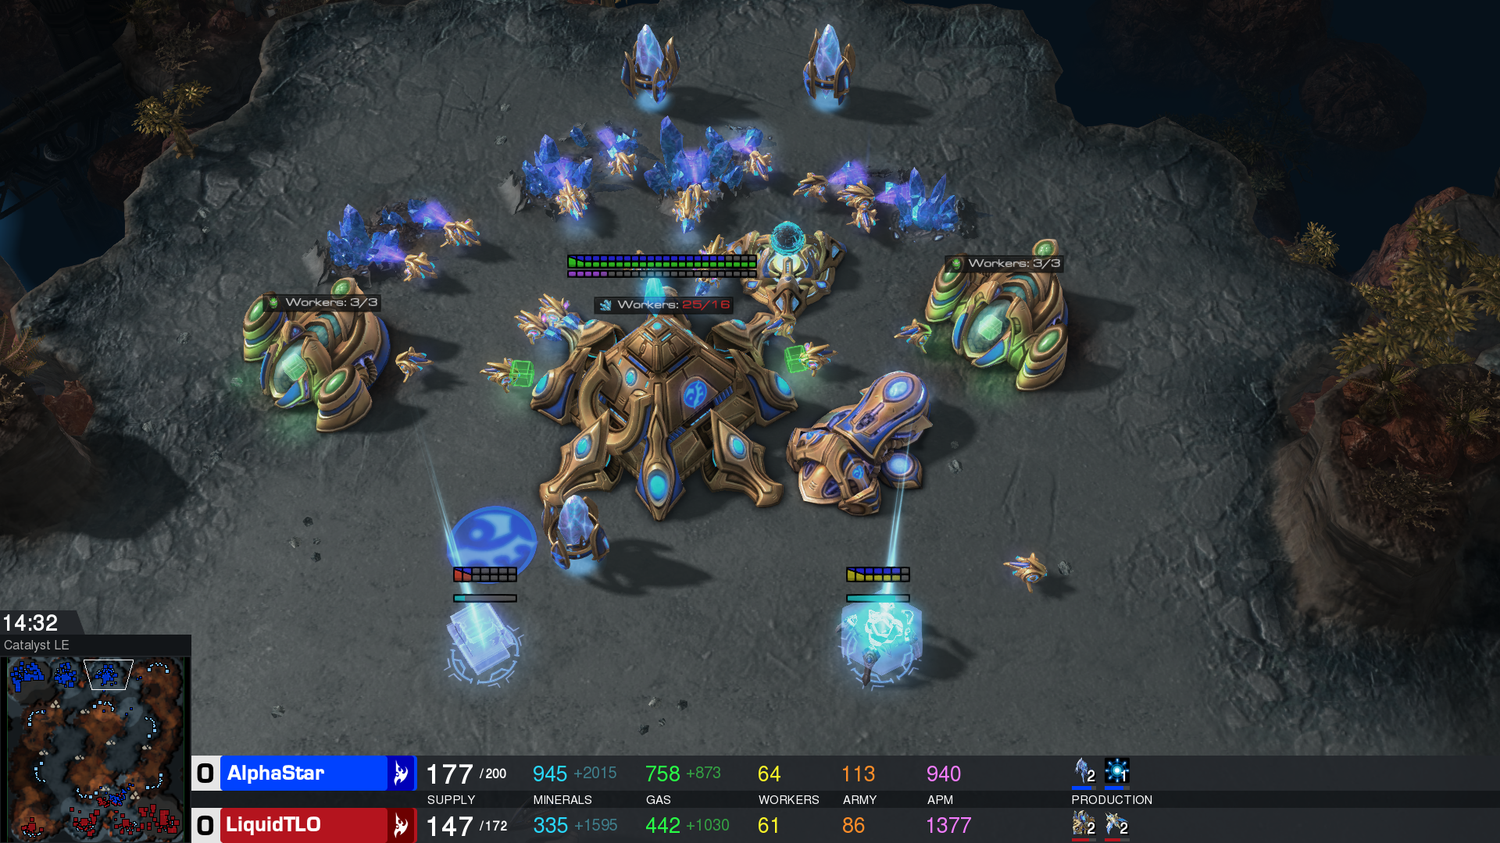
\includegraphics[width = 0.5\textwidth]{starcraft}
    \end{center}
    \caption{Vue de la base construite par AlphaStar pendant une des parties}
    \label{figure:starcraft}
\end{figure}
\FloatBarrier

AlphaStar est le premier programme à être capable de jouer à StarCraft II sans aucune modification des règles et directement depuis une vue brute des pixels du jeu.
Le programme est basé sur un réseau de neurones profond, entraîné utilisant un apprentissage par renforcement.

Un réseau de neurones est composé de plusieurs niveaux de neurones artificiels, ces niveaux sont reliés entre eux par l'équivalent, grandement simplifié, des synapses présentent dans notre cerveau.
Jusqu'à récemment, les réseaux de neurones dépassaient très rarement plus de 3 ou 4 niveaux, et ce, pour des raisons techniques.
Mais des découvertes ont permis d'augmenter ce nombre de niveaux à plusieurs dizaines~;~le principal facteur limitant étant actuellement la puissance de calcul nécessaire pour l'entraînement de ces réseaux.
Un réseau de neurones profond est donc un réseau de neurones utilisant des méthodes permettant d'augmenter sa profondeur, c'est-à-dire son nombre de niveaux.
Cela permet d'obtenir un système capable d'une grande abstraction et donc de montrer un raisonnement permettant de répondre à des problèmes très complexes.

StarCraft II est un jeu nécessitant de nombreuses optimisations à court terme qui se révèlent plus tard avoir un fort impact sur le long terme.
Le programme doit donc être capable de trouver un équilibre entre les objectifs à court et long terme et de s'adapter à des situations inattendues.
Contrairement à des jeux comme les échecs ou le jeu de go, StarCraft II nécessite de prendre des actions en temps réel et le joueur ne peut pas voir la totalité de son environnement à tout moment.
Les contraintes de ce jeu sont donc immenses et similaires aux contraintes auxquelles les êtres humains sont confrontés continuellement.
Développer un programme capable de s'adapter pour résoudre des situations comparables est donc une avancée scientifique de grande ampleur.

\subsubsection{Autres avancées de \textsc{DeepMind}}

La société \textsc{DeepMind} conduit de très nombreuses recherches dans le domaine de l'apprentissage profond, comme vu avec les deux précédentes sections.

On peut encore citer AlphaGo, le premier programme qui a battu un joueur humain professionnel et, par la même occasion, un champion du monde au jeu de Go, M. Fan \textsc{Hui}, en octobre 2015.
Ce programme fonctionne grâce à un réseau de neurones profond et une méthode d'apprentissage par renforcement.

En 2017, la compagnie introduit AlphaZero, un programme capable de jouer au jeu de Go, aux échecs et au shōgi (jeu de société japonais) à un niveau sans précédent sur chacun des jeux.

En 2018, \textsc{DeepMind} présente AlphaFold, programme fonctionnant aussi grâce à un réseau de neurones profond et qui permet, à partir d'une séquence de protéines, de déterminer un modèle 3D de la structure de la protéine résultante.
Cela à un fort intérêt pour les recherches scientifiques dans le domaine médical et notamment pour les recherches concernant les maladies d'Alzheimer ou de Parkinson par exemple.

\FloatBarrier
\begin{figure}[h!]
    \begin{minipage}[c]{0.55\textwidth}
        \begin{center}
            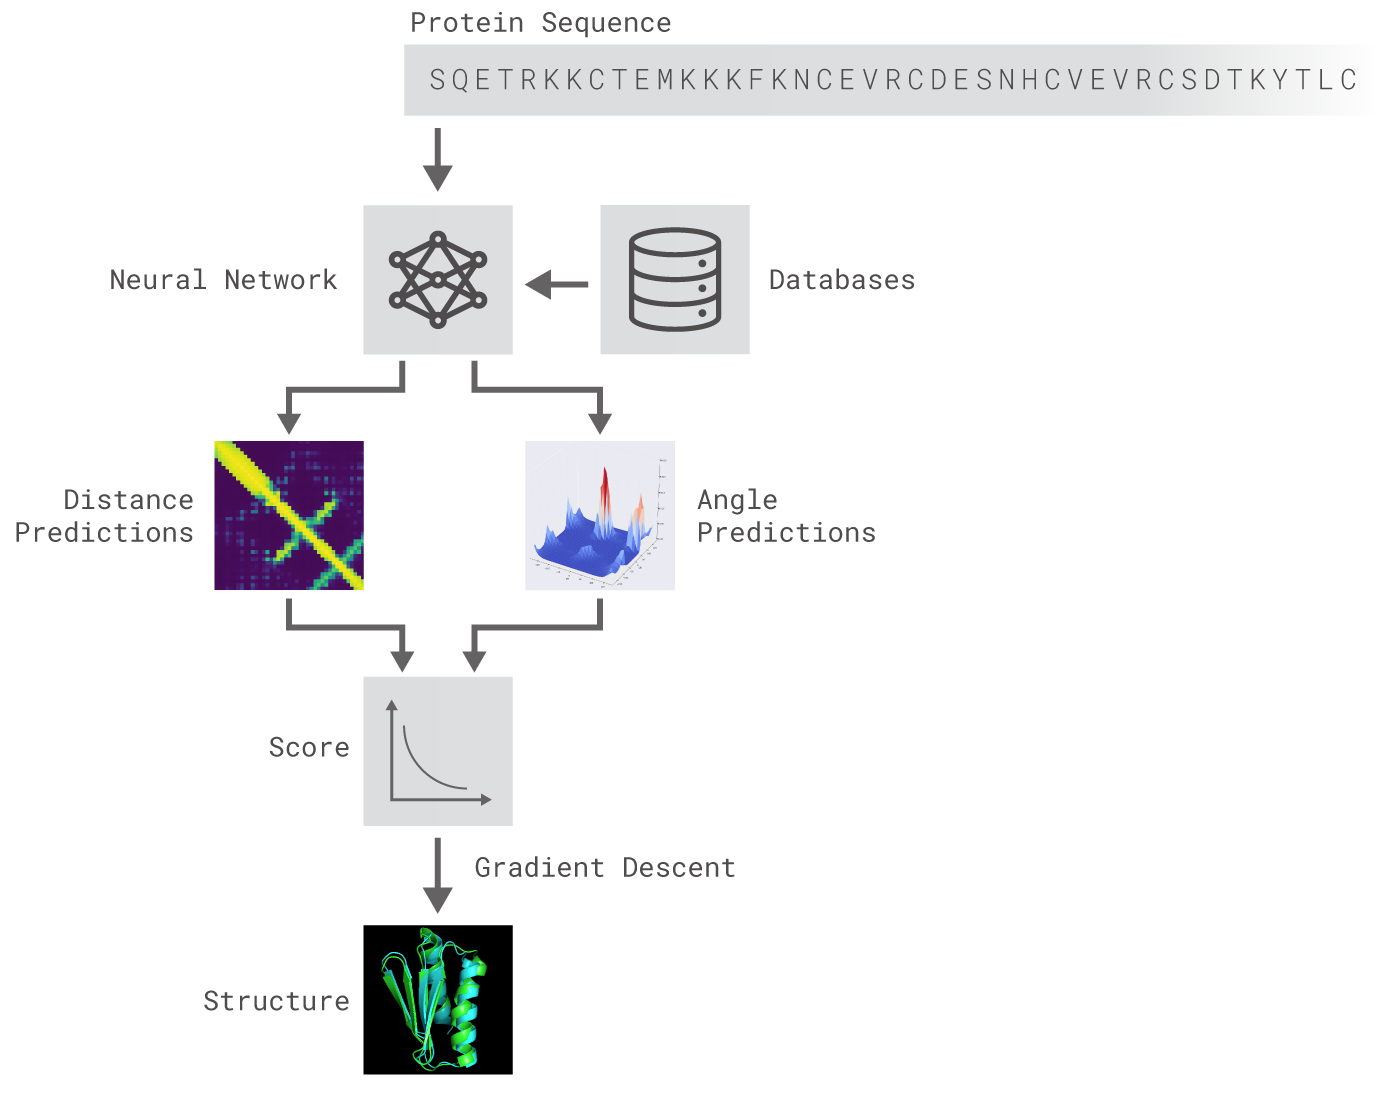
\includegraphics[width = \textwidth]{alphafold}
        \end{center}
    \end{minipage}\hfill
    \begin{minipage}[c]{0.45\textwidth}
        \caption{Fonctionnement d'AlphaFold pour la génération d'un modèle 3D d'une protéine à partir d'une séquence protéique}
        \label{figure:alphafold}
    \end{minipage}
\end{figure}
\FloatBarrier

\subsubsection{Pilote automatique de \textsc{Tesla} v9.0}

Depuis 2018, la dernière version du pilote automatique des véhicules de la marque \textsc{Tesla} est la version 9.0.
Elle suit la version 8.1.
Il est estimé qu'elle présente une augmentation des capacités de 400\% par rapport à la version précédente.
Il est complexe de trouver des informations sur le fonctionnement technique du programme de pilotage automatique de \textsc{Tesla}.
En effet, il ne s'agit pas ici d'expériences, comme pour la société \textsc{DeepMind}, mais d'un système utilisé à un niveau industriel et sur lequel la vie des utilisateurs dépend.

On sait tout de même que le pilote automatique est basé sur un réseau de neurones capable de prendre en compte les données recueillies par les huit caméras entourant le véhicule simultanément.
Il utilise un système de détection des objets très précis, ainsi il peut comprendre l'environnement du véhicule.

En termes de détection d'objets, segmentation d'images et reconnaissance d'images, les réseaux de neurones les mieux adaptés sont les réseaux neuronaux à convolution, il est donc très probable que le réseau du pilote automatique soit au moins partiellement de ce type.

Dans l'image ci-dessous on peut voir la détection des voitures et piétons ainsi que la segmentation de l'image effectuée pour détecter où se trouve la route à suivre.

\FloatBarrier
\begin{figure}[h!]
    \begin{center}
        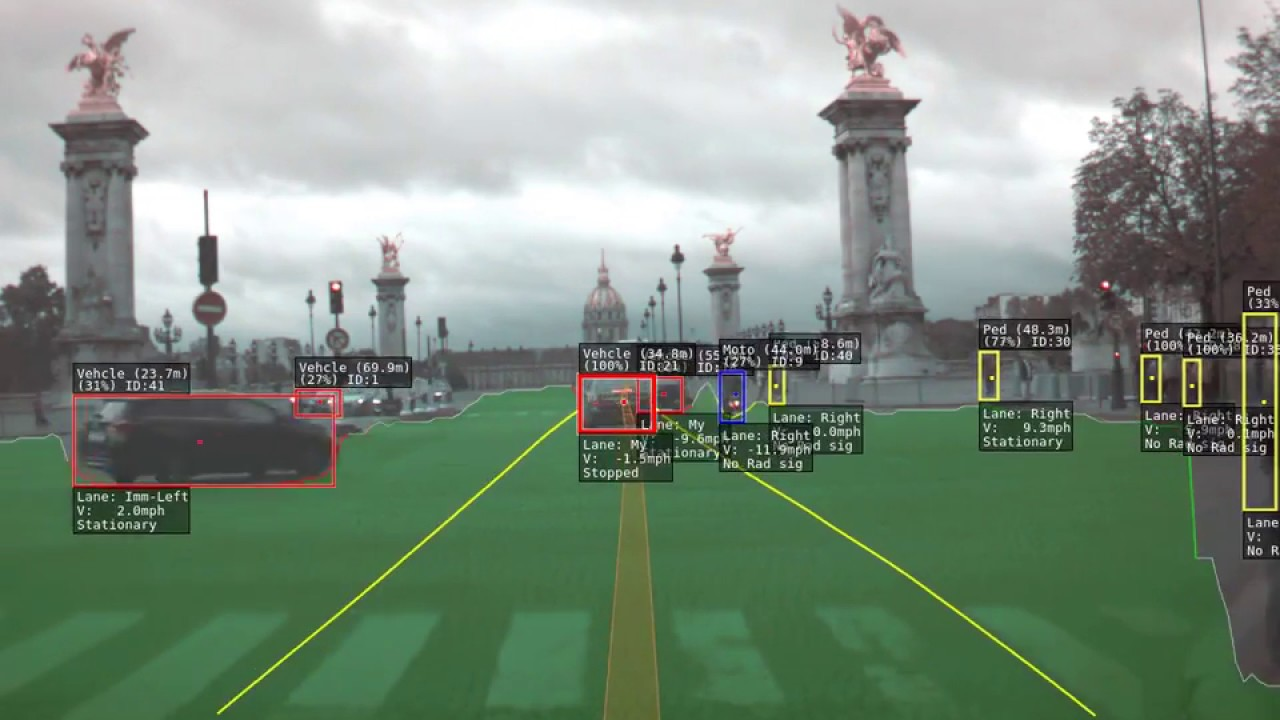
\includegraphics[width = 0.5\textwidth]{autopilot}
    \end{center}
    \caption{Visualisation de la détection d'objet du pilote automatique de \textsc{Tesla}}
    \label{figure:autopilot}
\end{figure}
\FloatBarrier

Les réseaux de neurones à convolution diffèrent des autres par l'utilisation d'un motif de connexion entre les neurones inspirés du cortex visuel des animaux.
C'est pour cette raison qu'ils sont si performants dans le traitement des images.

\subsubsection{GauGAN de \textsc{Nvidia}}

La société \textsc{Nvidia}, spécialisée dans la création de matériel informatique, réalise de nombreuses avancées dans le domaine de l'apprentissage profond.
En 2019, la compagnie a présenté et mis à disposition un outil permettant de transformer de simples croquis en paysage réaliste.
Sur l'image ci-dessous on peut voir le croquis sur la gauche et le paysage généré automatiquement sur la droite.

\FloatBarrier
\begin{figure}[h!]
    \begin{center}
        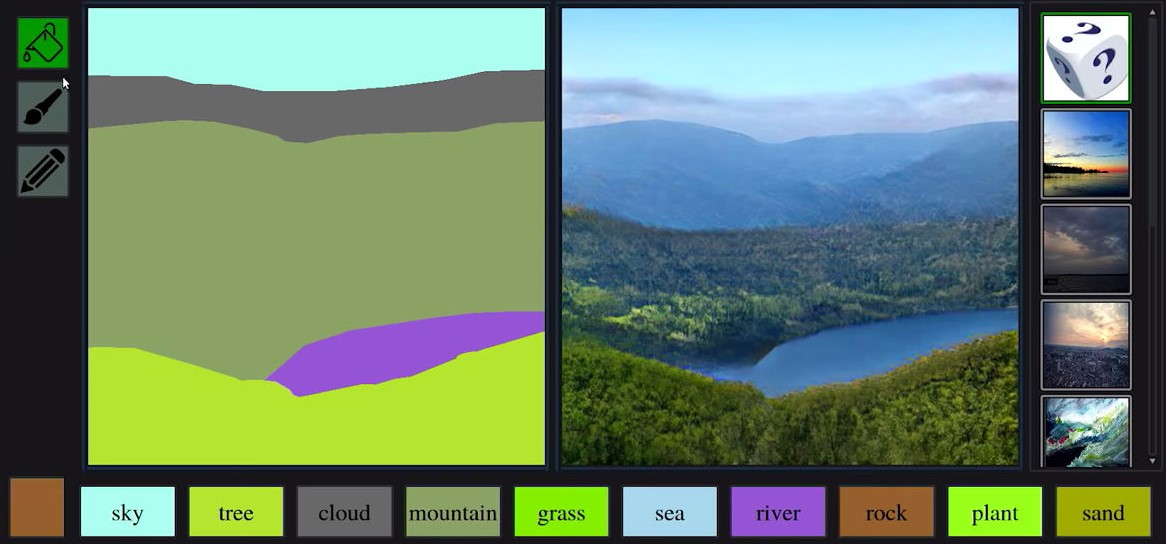
\includegraphics[width = 0.65\textwidth]{gaugan}
    \end{center}
    \caption{Transformation d'un dessin simpliste en paysage en utilisant GauGAN}
    \label{figure:gaugan}
\end{figure}
\FloatBarrier

Cet outil se base sur un concept récent de l'apprentissage profond : les <<~generative adversarial networks~>> (GAN), que l'on peut traduire par réseaux antagonistes génératifs.

Ce nouveau type d'algorithme fut introduit en 2014 \cite{gan}.
C'est un système dans lequel deux réseaux de neurones, généralement à convolution, sont placés en compétition, l'un est un générateur et l'autre est un discriminateur.
Le premier génère un échantillon, par exemple une image, le second essaye ensuite de déterminer si l'échantillon résulte du générateur ou est un échantillon réel.
L'entraînement d'un tel modèle a pour effet de permettre la génération d'échantillons très réalistes.
Les mises en application sont encore rares et relèvent généralement plus du domaine artistique que scientifique.

L'entreprise a aussi développé un outil permettant de faire disparaître un élément d'une photo automatiquement sur le même principe et l'a présenté par la même occasion.

D'un point de vue technique, il faut savoir que la meilleure manière d'entraîner un modèle d'apprentissage profond est de faire effectuer les calculs à une ou des carte(s) graphique(s), plutôt qu'à un ou des processeur(s).
Les cartes graphiques conviennent très bien à la réalisation de nombreux calculs en parallèle, contrairement aux processeurs, et donc conviennent parfaitement aux types de calculs requis lors de l'entraînement d'un réseau de neurones.
Les deux principaux producteurs de cartes graphiques au monde sont \textsc{Nvidia} et \textsc{Amd}.
C'est \textsc{Nvidia} qui s'est pour le moment le plus départagé par son investissement dans la recherche en apprentissage profond.
\textsc{Nvidia} a développé de nombreux outils permettant de grandement faciliter le développement de systèmes d'apprentissage profond sur ses cartes graphiques.
Ainsi, les chercheurs du domaine travaillent donc quasiment exclusivement avec cette compagnie.
